\documentclass{article}
\usepackage{tikz}
\usepackage{pdfpages}
\usepackage{amsmath}
\begin{document}
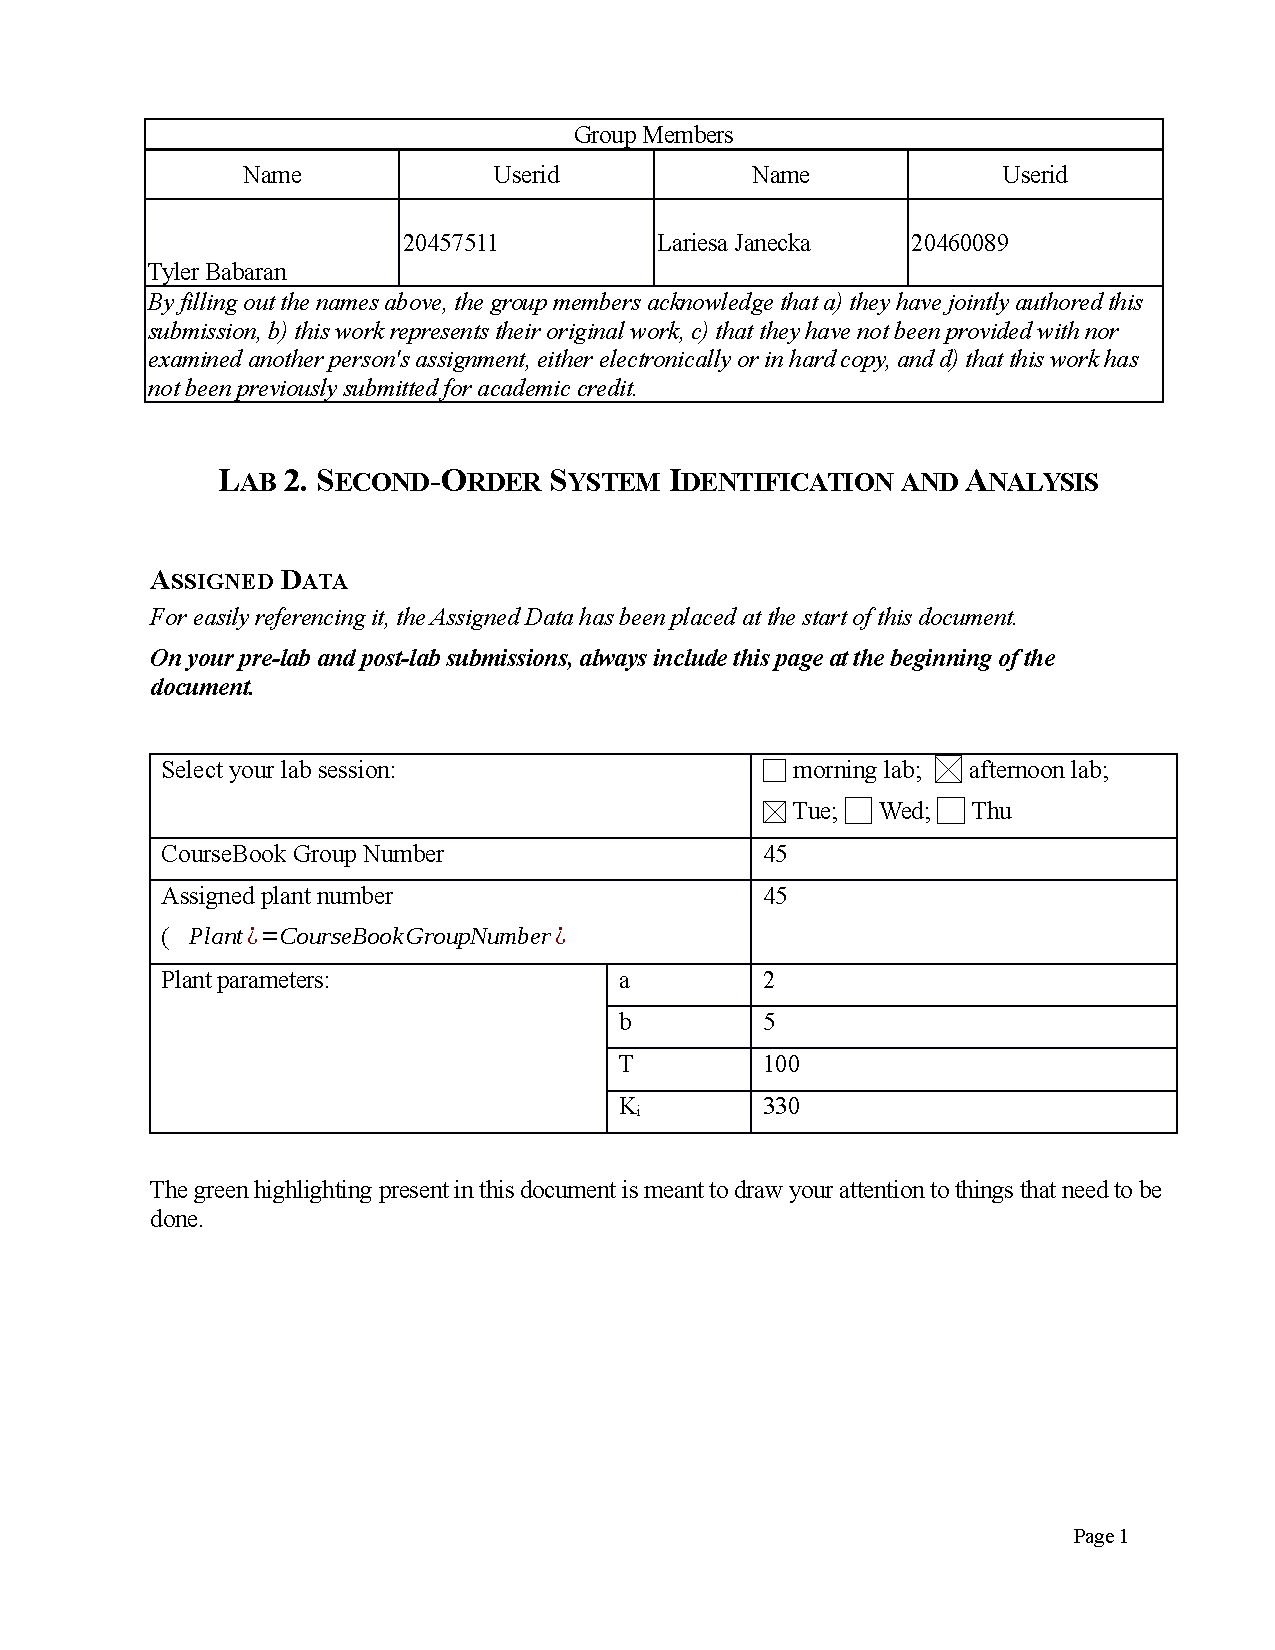
\includepdf[pages={1}]{page1.pdf}

\section*{Pre-Lab} % (fold)
\label{sec:pre_lab}

\subsection*{Question 1} % (fold)
\label{sub:question_1}
By reducing block diagram rules:
\begin{align*}
    \text{Let } H(S) &= \frac{K_i}{s}\times \frac{bT}{s+aT}\\
                    &= \frac{K_ibT}{s(s+aT)}\\
    G(S) &= \frac{H(S)}{1+ H(S)}\\
        &= \frac{\frac{K_ibT}{s(s+aT)}}{1+ \frac{K_ibT}{s(s+aT)}}\\
        &= \frac{\frac{K_ibT}{s(s+aT)}}{\frac{s(s+aT) + K_ibT}{s(s+aT)}}\\
        &= \frac{K_ibT}{s(s+aT)} \times \frac{s(s+aT)}{s(s+aT) + K_ibT}\\
        &= \frac{K_ibT}{s(s+aT) + K_ibT}\\
        &= \frac{K_ibT}{s^2 + aTs + K_ibT}\\
\end{align*}
% subsection question_1 (end)

\subsection*{Question 2} % (fold)
\label{sub:question_2}
Using the standard second order system.
\begin{align*}
G(S) &= \frac{\omega_n^2}{s^2 + 2\zeta\omega_ns + \omega_n^2}\\
\omega_n &= \sqrt{K_ibT}\\
2\zeta\omega_n &= aT\\
\zeta &= \frac{aT}{2\omega_n}\\
     &= \frac{aT}{2\sqrt{K_ibT}}\\
\end{align*}

% subsection question_2 (end)

\subsection*{Question 3} % (fold)
\label{sub:question_3}
%peak time = time at which the step response reaches its greatest value
% overshoot is the difference between the maximum and steady state values as a percentage of steady state
With OS in its decimal value.
\begin{align*}
T_p &= \frac{\pi}{\omega_n\sqrt{1-\zeta^2}}\\
OS &= e^{\frac{-\zeta\pi}{\sqrt{1- \zeta^2}}}\\
\ln{OS} &= \frac{-\zeta\pi}{\sqrt{1- \zeta^2}}\\
\ln{OS} \times \sqrt{1- \zeta^2} &= -\zeta\pi\\
\ln^2{OS} \times (1- \zeta^2) &= \zeta^2\pi^2\\
\ln^2{OS} - \ln^2{OS}\zeta^2 &= \zeta^2\pi^2\\
\ln^2{OS}  &= \zeta^2(\ln^2{OS} + \pi^2)\\
\zeta &= \sqrt{\frac{\ln^2{OS}}{\ln^2{OS} + \pi^2}}\\
\end{align*}

% subsection question_3 (end)

\subsection*{Question 4a} % (fold)
\label{sub:question_4a}

\begin{align*}
    H_{open}(S) &= (K_p \times G(S) + D(S)) \times K\\
         &= G(S)\\
         &= \frac{K_ibT}{s^2 + aTs + K_ibT}\\
\end{align*}

% subsection question (end)

\subsection*{Question 4b} % (fold)
\label{sub:question_4b}
\begin{align*}
    H_{closed}(S) &=  \frac{H_{open}(S)}{1 + H_{open}(S)}\\
         &= \frac{\frac{K_ibT}{s^2 + aTs + K_ibT}}{1 + \frac{K_ibT}{s^2 + aTs + K_ibT}}\\
         &= \frac{\frac{K_ibT}{s^2 + aTs + K_ibT}}{\frac{s^2 + aTs + K_ibT + K_ibT}{s^2 + aTs + K_ibT}}\\
         &= \frac{K_ibT}{s^2 + aTs + K_ibT} \times \frac{s^2 + aTs + K_ibT}{s^2 + aTs + 2K_ibT}\\
         &= \frac{K_ibT}{s^2 + aTs + 2K_ibT}\\
\end{align*}
% subsection question_4b (end)

\subsection*{Question 4c} % (fold)
\label{sub:question_4c}
\begin{align*}
    H_d(S) &= \frac{K}{1 + K\times (R(S) + K_p \times G(S))}\\
    H_d(S) &= \frac{1}{1 + G(S)}\\
    H_d(S) &= \frac{1}{1 + \frac{K_ibT}{s^2 + aTs + K_ibT}}\\
    H_d(S) &= \frac{1}{\frac{s^2 + aTs + K_ibT + K_ibT}{s^2 + aTs + K_ibT}}\\
    H_d(S) &= \frac{s^2 + aTs + K_ibT}{s^2 + aTs + 2K_ibT}\\
\end{align*}
% subsection question_4c (end)

\subsubsection*{Question 5} % (fold)
\label{ssub:question_5}
\begin{tabular}{|l|l|l|}
    \hline
    \textbf{Assigned Parameter Value} & \textbf{Select Range Value} & \textbf{ACS13016 Display Value}\\
    \hline
    2 & - & 20 \\
    \hline
    5 & - & 50 \\
    \hline
    330 & 10 & 33\\
    \hline
\end{tabular}
% subsubsection question_5 (end)

% section pre_lab (end)



\end{document}
